\let\negmedspace\undefined
\let\negthickspace\undefined
\documentclass[journal]{IEEEtran}
\usepackage[a5paper, margin=10mm, onecolumn]{geometry}
%\usepackage{lmodern} % Ensure lmodern is loaded for pdflatex
\usepackage{tfrupee} % Include tfrupee package

\setlength{\headheight}{1cm} % Set the height of the header box
\setlength{\headsep}{0mm}     % Set the distance between the header box and the top of the text

\usepackage{gvv-book}
\usepackage{gvv}
\usepackage{cite}
\usepackage{amsmath,amssymb,amsfonts,amsthm}
\usepackage{algorithmic}
\usepackage{graphicx}
\usepackage{textcomp}
\usepackage{xcolor}
\usepackage{txfonts}
\usepackage{listings}
\usepackage{enumitem}
\usepackage{mathtools}
\usepackage{gensymb}
\usepackage{comment}
\usepackage[breaklinks=true]{hyperref}
\usepackage{tkz-euclide} 
\usepackage{listings}
% \usepackage{gvv}                                        
\def\inputGnumericTable{}                                 
\usepackage[latin1]{inputenc}                                
\usepackage{color}                                            
\usepackage{array}                                            
\usepackage{longtable}                                       
\usepackage{calc}                                             
\usepackage{multirow}                                         
\usepackage{hhline}                                           
\usepackage{ifthen}                                           
\usepackage{lscape}
\begin{document}

\bibliographystyle{IEEEtran}
\vspace{3cm}




\title{
%	\logo{
GATE - 2008 - EE

\large{EE1030 : Matrix Theory}

Indian Institute of Technology Hyderabad
%	}
}
\author{Satyanarayana Gajjarapu

AI24BTECH11009
}	





\maketitle




\bigskip

\renewcommand{\thefigure}{\theenumi}
\renewcommand{\thetable}{\theenumi}


\section{1 - 17}

\begin{enumerate}
\item The number of chords in the graph of the given circuit will be
\begin{figure}[!ht]
\centering
\resizebox{0.5\textwidth}{!}{%
\begin{circuitikz}
\tikzstyle{every node}=[font=\normalsize]
\draw [short] (6.5,11.75) -- (6.5,8.25);
\draw [short] (4,10) -- (9,10);
\draw  (6.5,10) circle (1.25cm);
\node at (7,10.5) [circ] {};
\node [font=\normalsize] at (7.25,10.5) {$z$};
\node [font=\normalsize] at (6.75,12) {Im};
\node [font=\normalsize] at (9,9.75) {Re};
\node [font=\normalsize] at (8,11.75) {Unit circle};
\draw [->, >=Stealth] (7.5,11.5) -- (7.25,11.25);
\end{circuitikz}

}%
\end{figure}
    \begin{enumerate}
        \item 3
        \item 4
        \item 5
        \item 6 \\
    \end{enumerate}
\item The Thevenin's equivalent of a circuit operating at $\omega$ = 5 rad/s, has $V_{oc} = 3.71\angle{-15.9\degree} V$ and $Z_o = 2.38 - j0.667\Omega$. At this frequency, the minimal realization of the Thevenin's impedance will have a
\begin{enumerate}
    \item resistor and a capacitor and an inductor
    \item resistor and a capacitor
    \item resistor and an inductor
    \item capacitor and an inductor \\
\end{enumerate}
\item A signal $e^{-\alpha t}\sin\brak{\omega t}$ is the input to a real Linear Time Invariant system. Given $K$ and $\phi$ are constants, the output of the system will be of the form $Ke^{-\beta t}\sin\brak{vt+\phi}$ where
\begin{enumerate}
    \item $\beta$ need not be equal to $\alpha$ but $v$ equal to $\omega$
    \item $v$ need not be equal to $\omega$ but $\beta$ equal to $\alpha$
    \item $\beta$ equal to $\alpha$ and $v$ is equal to $\omega$
    \item $\beta$ need not be equal to $\alpha$ and $v$ need not be equal to $\omega$ \\
\end{enumerate}
\item $X$ is a uniformly distributed random variable that takes values between 0 and 1. The value of $E\{X^3\}$ will be
 \begin{enumerate}
     \item 0
     \item $\frac{1}{8}$
     \item $\frac{1}{4}$
     \item $\frac{1}{2}$ \\
 \end{enumerate}
\item The characteristic equation of a $\brak{3 \times 3}$ matrix $\vec{P}$ is defined as 
\begin{align*}
    \alpha\brak{\lambda} = \abs{\lambda\vec{I} - \vec{P}} = \lambda^3 + \lambda^2 + 2\lambda + 1 = 0
\end{align*}
If $\vec{I}$ denotes identity matrix, then the inverse of matrix $\vec{P}$ will be
\begin{enumerate}
    \item $\brak{\vec{P}^2 + \vec{P} + \vec{2I}}$
    \item $\brak{\vec{P}^2 + \vec{P} + \vec{I}}$
    \item $-\brak{\vec{P}^2 + \vec{P} + \vec{I}}$
    \item $-\brak{\vec{P}^2 + \vec{P} + \vec{2I}}$ \\
\end{enumerate}
\item If the rank of a \brak{5 \times 6} matrix $\vec{Q}$ is 4, then which one of the following statements is correct?
\begin{enumerate}
    \item $\vec{Q}$ will have four linearly independent rows and four linearly independent columns
    \item $\vec{Q}$ will have four linearly independent rows and five linearly independent columns
    \item $\vec{Q Q^\intercal}$ will be invertible
    \item $\vec{Q^\intercal Q}$ will be invertible \\
\end{enumerate}
\item A function $y\brak{t}$ satisfies the following differential equation:
\begin{align*}
    \frac{dy\brak{t}}{dt} + y\brak{t} = \delta\brak{t}
\end{align*}
where $\delta\brak{t}$ is the delta function. Assuming zero initial condition, and denoting the unit step function by $u\brak{t}$, $y\brak{t}$ can be of form
\begin{enumerate}
    \item $e^t$
    \item $e^{-t}$
    \item $e^tu\brak{t}$
    \item $e^{-t}u\brak{t}$ \\
\end{enumerate}
\item The equivalent circuits of a diode, during forward biased and reverse biased conditions, are shown in the figure
\begin{figure}[!ht]
\centering
\resizebox{0.5\textwidth}{!}{%
\begin{circuitikz}
\tikzstyle{every node}=[font=\large]
\draw (2.5,11.25) to[D] (5.25,11.25);
\draw (2.5,10) to[D] (5.25,10);
\node [font=\LARGE] at (6.5,11.25) {$\equiv$};
\node [font=\LARGE] at (6.5,10) {$\equiv$};
\node [font=\normalsize] at (2.5,11.5) {+};
\node [font=\normalsize] at (5.25,10.25) {+};
\node [font=\normalsize] at (5.25,11.5) {-};
\node [font=\normalsize] at (2.5,10.25) {-};
\draw (4.5,11.25) to[short, -o] (5.25,11.25) ;
\draw (4.5,10) to[short, -o] (5.25,10) ;
\draw (3,11.25) to[short, -o] (2.5,11.25) ;
\draw (2.75,10) to[short, -o] (2.5,10) ;
\draw (7.75,11.25) to[battery1] (9.5,11.25);
\draw (9.5,11.25) to[R] (11.25,11.25);
\draw (7.75,10) to[normal open switch] (11.25,10);
\draw (8,11.25) to[short, -o] (7.75,11.25) ;
\draw (8,10) to[short, -o] (7.75,10) ;
\draw (11,11.25) to[short, -o] (11.25,11.25) ;
\node [font=\large] at (8.75,11.75) {$0.7 V$};
\draw (11,10) to[short, -o] (11.25,10) ;
\node [font=\large] at (10.5,11.75) {$R_d$};
\end{circuitikz}

}%
\end{figure}\\
\begin{figure}[!ht]
\centering
\resizebox{0.5\textwidth}{!}{%
\begin{circuitikz}
\tikzstyle{every node}=[font=\large]
\draw (3,11.25) to[sinusoidal voltage source, sources/symbol/rotate=auto] (3,8.75);
\draw (3,11.25) to[R] (6,11.25);
\node at (6,11.25) [circ] {};
\draw (6,11.25) to[short] (8.25,11.25);
\draw (8.25,11.25) to[R] (8.25,8.75);
\draw (6,11.25) to[D] (6,9.5);
\draw (6,9.5) to[battery1] (6,8.75);
\node at (6,8.75) [circ] {};
\draw (3,8.75) to[short] (8.25,8.75);
\node [font=\large] at (4.5,11.75) {10 k$\Omega$};
\node [font=\large] at (1.65,10) {10 Sin$\brak{\omega t}$};
\node [font=\large] at (6.75,9.25) {$5 V$};
\node [font=\large] at (9,10) {$10 k\Omega$};
\node [font=\large] at (7.75,10.25) {$v_o$};
\node [font=\large] at (7.75,10.75) {$\uparrow$};
\draw [short] (7.75,10) -- (7.75,9.25);
\end{circuitikz}

}%
\end{figure}
\\
If such a diode is used in clipper circuit of figure given above, the output voltage $\brak{v_o}$ of the circuit will be 
 \begin{enumerate}
     \item 
      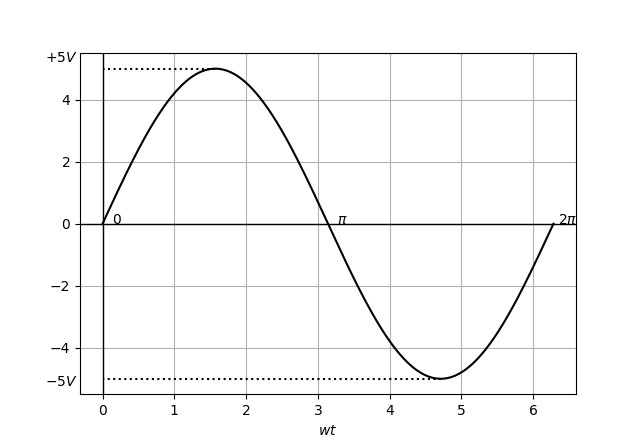
\includegraphics[width=0.3\linewidth]{figs/A8.1.png}
        \item 
\resizebox{0.3\textwidth}{!}{%
\begin{circuitikz}
\tikzstyle{every node}=[font=\normalsize]
\draw [->, >=Stealth] (7,11.5) -- (7,16.25);
\draw [->, >=Stealth] (7,13.75) -- (12.75,13.75);
\draw [short] (7,13.75) -- (7.75,15);
\draw [short] (7.75,15) .. controls (8.25,15.25) and (8.25,15.25) .. (8.75,15);
\draw [short] (8.75,15) -- (9.5,13.75);
\draw [short] (9.5,13.75) .. controls (10.25,11.5) and (10.75,12) .. (11.25,13.75);
\draw [dashed] (7.75,15) -- (8.75,15);
\draw [dashed] (7,12.25) -- (10.5,12.25);
\node [font=\normalsize] at (12.75,13.5) {$\omega$t};
\node [font=\normalsize] at (6.25,15) {5.7 V};
\node [font=\normalsize] at (6.25,12.25) {-10 V};
\node [font=\normalsize] at (11.5,14) {2$\pi$};
\node [font=\normalsize] at (9.75,14) {$\pi$};
\node [font=\normalsize] at (6.75,14) {0};
\end{circuitikz}


}%
     \item 
      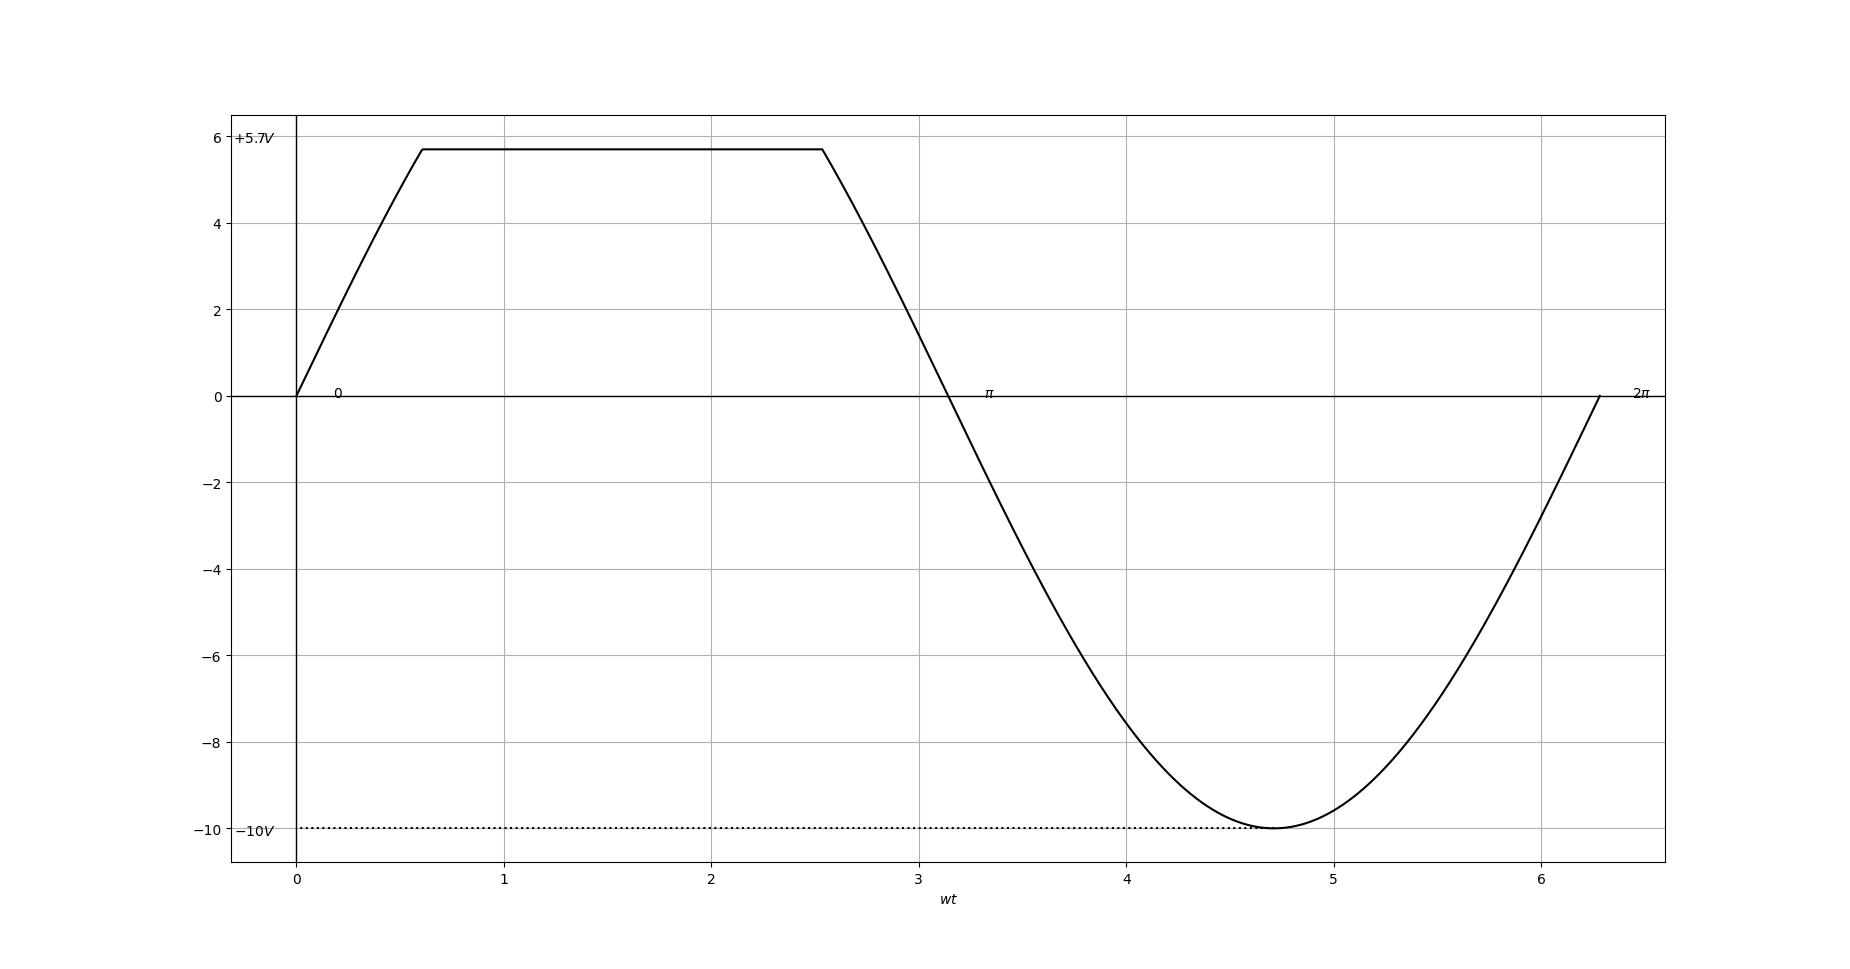
\includegraphics[width=0.3\linewidth]{figs/A8.3.png}
     \item 
\resizebox{0.3\textwidth}{!}{%
\begin{circuitikz}
\tikzstyle{every node}=[font=\normalsize]
\draw [->, >=Stealth] (7,11.5) -- (7,16.25);
\draw [->, >=Stealth] (7,13.75) -- (12.75,13.75);
\node [font=\normalsize] at (12.75,13.5) {$\omega$ t};
\node [font=\normalsize] at (11.5,14) {2$\pi$};
\node [font=\normalsize] at (9.75,14) {$\pi$};
\node [font=\normalsize] at (6.75,14) {0};
\draw [short] (7,13.75) .. controls (8.5,16.5) and (8.5,15) .. (9.75,13.75);
\draw [short] (9.75,13.75) -- (10.25,12.5);
\draw [short] (11.5,13.75) -- (11,12.5);
\draw [short] (10.25,12.5) .. controls (10.75,12.25) and (10.75,12.25) .. (11,12.5);
\draw [dashed] (7,12.5) -- (11,12.5);
\node [font=\normalsize] at (6.25,15.25) {10 V};
\node [font=\normalsize] at (6.5,12.5) {-5.7 V};
\end{circuitikz}


}%

 \end{enumerate}
\item Two 8-bit ADCs, one of single slope integrating type and the other of successive approximation type, take $T_A$ and $T_B$ times to convert a 5 V analog input signal to an equivalent digital output. If the input analog signal is reduced to 2.5 V, the approximate time taken by the two ADCs will respectively, be
\begin{enumerate}
     \item $T_A, T_B$
     \item $\frac{T_A}{2}, T_B$
     \item $T_A, \frac{T_B}{2}$
     \item $\frac{T_A}{2}, \frac{T_B}{2}$ \\
 \end{enumerate}
\item An input device is interfaced with Intel 8085A microprocessor as memory mapped I/O. The address of the device is 2500H. In order to input data from the device to accumulator, the sequence of instructions will be
\begin{enumerate}
    \item LXI\ \ \ H, 2500H \\
    MOV A, M
    \item LXI\ \ \ H, 2500H \\
    MOV M, A
    \item LHLD 2500H \\
    MOV A, M
    \item LHLD 2500H \\
    MOV M, A \\
\end{enumerate}
\item Distributed winding and short chording employed in AC machines will result in
\begin{enumerate}
    \item increase in emf and reduction in harmonics.
    \item reduction in emf and increase in harmonics.
    \item increase in both emf and harmonics.
    \item reduction in both emf and harmonics. \\
\end{enumerate}
\item Three single-phase transformers are connected to form a 3-phase transformer bank. The transformers are connected in the following manner:\\
\begin{figure}[!ht]
\centering
\resizebox{0.5\textwidth}{!}{%
\begin{tabular}[12pt]{ |c| c| c| c|}
    \hline
    \textbf{Combination choice} & \textbf{Phase I} & \textbf{Phase II} & \textbf{Phase III} \\ 
    \hline
    P & 1, 4 & 2, 5 & 3, 6 \\
    \hline 
    Q & 1, 2 & 4, 5 & 3, 6 \\
    \hline
    R & 2, 5 & 1, 3 & 4, 6 \\
    \hline
    S & 1, 4 & 2, 6 & 3, 5 \\
    \hline
    \end{tabular}

}%
\end{figure}\\
The transformer connection will be represented by
\begin{enumerate}
    \item Yd0
    \item Yd1
    \item Yd6
    \item Yd11 \\
\end{enumerate}
\item In a stepper motor, the detent torque means
\begin{enumerate}
    \item minimum of the static torque with the phase winding excited.
    \item maximum of the static torque with the phase winding excited.
    \item minimum of the static torque with the phase winding unexcited.
    \item maximum of the static torque with the phase winding unexcited. \\
\end{enumerate}
\item A two machine power system is shown below. Transmission line $XY$ has positive sequence impedance of $Z_1 \Omega$ and zero sequence impedance of $Z_0 \Omega$. 
\pagebreak
\begin{figure}[!ht]
\centering
\resizebox{0.5\textwidth}{!}{%
\begin{circuitikz}
\tikzstyle{every node}=[font=\normalsize]
\draw (6.75,14.25) to[short] (14.5,14.25);
\draw (8.75,15) to[short] (8.75,13.5);
\draw (12.75,15) to[short] (12.75,13.5);
\draw  (6.25,14.25) circle (0.5cm);
\draw  (15,14.25) circle (0.5cm);
\draw [short] (10.5,14.25) -- (10.25,14);
\draw [short] (10.25,14) -- (10.75,14);
\draw [->, >=Stealth] (10.75,14) -- (10.25,13.5);
\node [font=\normalsize] at (11,14) {F};
\node [font=\normalsize] at (8.75,15.25) {X};
\node [font=\normalsize] at (12.75,15.25) {Y};
\node [font=\normalsize] at (6.25,14.25) {$\sim$};
\node [font=\normalsize] at (15,14.25) {$\sim$};
\end{circuitikz}


}%
\end{figure} \\
An '$a$' phase to ground fault with zero fault impedance occurs at the centre of the transmission line. Bus voltage at $X$ and line current from $X$ to $F$ for the phase '$a$', are given by $V_a$ Volts and $I_a$ Amperes, respectively. Then, the impedance measured by the ground distance relay located at the terminal $X$ of line $XY$ will be given by
\begin{enumerate}
   \item $\frac{Z_1}{2} \Omega$
   \item $\frac{Z_0}{2} \Omega$
   \item $\frac{Z_0+Z_1}{2} \Omega$
   \item $\frac{V_a}{I_a} \Omega$ \\
\end{enumerate}
\item An extra high voltage transmission line of length 300 km can be approximated by a lossless line having propagation constant $\beta$ = 0.00127 radians per km. Then the percentage ratio of line length to wavelength will be given by
\begin{enumerate}
    \item 24.24\%
    \item 12.12\%
    \item 19.05\%
    \item 6.06\% \\
\end{enumerate}
\item A 3-phase transmission line is shown in the figure:\\
\begin{figure}[!ht]
\centering
\resizebox{0.3\textwidth}{!}{%
\begin{circuitikz}
\tikzstyle{every node}=[font=\normalsize]
\draw [short] (3.25,11.5) -- (3.25,10.75);
\draw [short] (3.25,11) -- (8,11);
\draw [short] (8,11.5) -- (8,10.75);
\node [font=\normalsize] at (5.5,11.5) {$\Delta V_a$};
\draw [->, >=Stealth] (6,11.5) -- (7.75,11.5);
\draw [->, >=Stealth] (5,11.5) -- (3.5,11.5);
\draw [->, >=Stealth] (4.5,11) -- (6.75,11);
\node [font=\normalsize] at (6.75,10.75) {$I_a$};
\end{circuitikz}

}%
\end{figure}
\begin{figure}[!ht]
\centering
\resizebox{0.3\textwidth}{!}{%
\begin{circuitikz}
\tikzstyle{every node}=[font=\normalsize]
\draw [short] (3.25,11.5) -- (3.25,10.75);
\draw [short] (3.25,11) -- (8,11);
\draw [short] (8,11.5) -- (8,10.75);
\node [font=\normalsize] at (5.5,11.5) {$\Delta V_b$};
\draw [->, >=Stealth] (6,11.5) -- (7.75,11.5);
\draw [->, >=Stealth] (5,11.5) -- (3.5,11.5);
\draw [->, >=Stealth] (4.5,11) -- (6.75,11);
\node [font=\normalsize] at (6.75,10.75) {$I_b$};
\end{circuitikz}

}%
\end{figure}
\begin{figure}[!ht]
\centering
\resizebox{0.3\textwidth}{!}{%
\begin{circuitikz}
\tikzstyle{every node}=[font=\normalsize]
\draw [short] (3.25,11.5) -- (3.25,10.75);
\draw [short] (3.25,11) -- (8,11);
\draw [short] (8,11.5) -- (8,10.75);
\node [font=\normalsize] at (5.5,11.5) {$\Delta V_c$};
\draw [->, >=Stealth] (6,11.5) -- (7.75,11.5);
\draw [->, >=Stealth] (5,11.5) -- (3.5,11.5);
\draw [->, >=Stealth] (4.5,11) -- (6.75,11);
\node [font=\normalsize] at (6.75,10.75) {$I_c$};
\end{circuitikz}

}%
\end{figure}\\
Voltage drop across the transmission line is given by the following equation:
\begin{align*}
    \sbrak{\begin{matrix}
        \Delta V_a \\ \Delta V_b \\ \Delta V_c
    \end{matrix}} = \sbrak{\begin{matrix}
        Z_s & Z_m & Z_m \\Z_m & Z_s & Z_m \\ Z_m & Z_m & Z_s
    \end{matrix}}\sbrak{\begin{matrix}
        I_a \\ I_b \\ I_c
    \end{matrix}}
\end{align*}
Shunt capacitance of the line can be neglected. If the line has positive sequence impedance of 15 $\Omega$ ans zero sequence impedance of 48 $\Omega$, then the values of $Z_s$ and $Z_m$ will be
\begin{enumerate}
    \item $Z_s=31.5\ \Omega$; $Z_m=16.5\ \Omega$
    \item $Z_s=26\ \Omega$; $Z_m=11\ \Omega$
    \item $Z_s=16.5\ \Omega$; $Z_m=31.5\ \Omega$
    \item $Z_s=11\ \Omega$; $Z_m=26\ \Omega$ \\
\end{enumerate}
\item In the single phase voltage controller circuit shown in the figure, for what range of triggering angle $\brak{\alpha}$, the output voltage $\brak{v_0}$ is not controllable?
\begin{figure}[!ht]
\centering
\resizebox{0.5\textwidth}{!}{%
\begin{circuitikz}
\tikzstyle{every node}=[font=\normalsize]
\draw (3.75,10.5) to[sinusoidal voltage source, sources/symbol/rotate=auto] (3.75,8);
\draw (5,10.5) to[D] (7.25,10.5);
\draw (7.25,9.25) to[D] (5,9.25);
\draw (3.75,10.5) to[short] (5.25,10.5);
\draw (7.25,10.5) to[short] (9.25,10.5);
\draw (7.25,10.5) to[short] (7.25,9.25);
\draw (5,10.5) to[short] (5,9.25);
\node at (5,10.5) [circ] {};
\node at (7.25,10.5) [circ] {};
\draw (9.25,10.5) to[R] (9.25,8.75);
\draw (9.25,8.75) to[L ] (9.25,7.25);
\draw (3.75,8) to[short] (3.75,7.25);
\draw (3.75,7.25) to[short] (9.25,7.25);
\node [font=\large] at (10,9.75) {$50 \Omega$};
\node [font=\large] at (10.25,8) {$j50\Omega$};
\node [font=\normalsize] at (3.1,9.25) {$v_s$};
\node [font=\normalsize] at (3.5,9.75) {$+$};
\node [font=\normalsize] at (3.5,8.75) {$-$};
\node [font=\normalsize] at (8.75,9) {$v_o$};
\draw [->, >=Stealth] (8.75,9.25) -- (8.75,10.25);
\draw [short] (8.75,8.75) -- (8.75,7.5);
\end{circuitikz}

}%
\end{figure}
\begin{enumerate}
    \item $0\degree < \alpha < 45\degree$
    \item $45\degree < \alpha < 135\degree$
    \item $90\degree < \alpha < 180\degree$
    \item $135\degree < \alpha < 180\degree$ \\
\end{enumerate}
			 \end{enumerate}
			 \end{document}

